\documentclass[12pt,a4paper]{article}  % Déclare la classe du document.

%  ------------------------------------------  Modules usuels  --------------------------------------
%  --------------------------------------------------------------------------------------------------------

\usepackage{amsmath} 	
\usepackage{amssymb} 
\usepackage{listings}         
\usepackage{numprint} 
\usepackage{pifont}

%  --------------------------------------------------------------------------------------------------------
% ----------------------  packages pour fontes et caractères spéciaux  ---------------------
%  --------------------------------------------------------------------------------------------------------

\usepackage{eurosym}   
\usepackage{amsfonts}   
\usepackage{amstext}       
\usepackage{amsfonts}	
\usepackage{mathrsfs}	 

\usepackage{pstricks,pst-all,pstricks-add,pst-tree,pst-node,pst-3dplot}

%------------------------------------------------------------------------------------------------------
%  --------------------------  Francisation et gestion des caractères sous mac --------------------------------------------------------------------------------------------------------

\usepackage[francais]{babel}   
\usepackage[utf8]{inputenc}
\usepackage[OT1,T1]{fontenc} 
%  --------------------------------------------------------------------------------------------------------
% ------------------------------------Packages  de  mise en page ---------------------------
%--------------------------------------------------------------------------------------------------------

\usepackage{fancyhdr}	% en-têtes et pieds de pages
\usepackage{amsfonts}

 \usepackage{multicol} % permet l'utilisation du multicolonnage dans le texte. La syntaxe est \begin{multicols}{nb de colonnes}    ......  \end{multicols}
 
\usepackage{calc}            % permet de faire un minimum de calcul sur les arguments des commandes et macros (utilisé dans la def de l'environnement preuve )
\usepackage{epic}            % extension et simplification de  l'environnement picture
\usepackage{graphicx}    % permet d'inclure des graphique externe dans un document
\usepackage{variations}   % permet d'obtenir de joli tableau de variations
\usepackage{enumerate}  %permet de faire des listes personnalisées
\usepackage{arydshln}     %permet d'avoir des lignes en pointillés
\usepackage{framed}  
\usepackage{multido} 


%  --------------------------------------  MACROS USUELLES  ----------------------------------------

\newcommand{\R}{\mathbb{R}} 
\newcommand{\N}{\mathbb{N}} 
\newcommand{\D}{\mathbb{D}} 
\newcommand{\Z}{\mathbb{Z}} 
\newcommand{\Q}{\mathbb{Q}} 
\newcommand{\C}{\mathbb{C}} 

%  -------------------------------------  MACROS SPECIFIQUES ------------------------------------


\newcommand{\raisedrule}[2][0em]{\leaders\hbox{\rule[#1]{1pt}{#2}}\hfill}


\newcounter{numexo}

\setcounter{numexo}{1}

\newcommand{\exercice}[1]{\vskip 0.6cm\noindent\rule[+2pt]{1cm}{0.5pt}\ {\large\bf \ Exercice \thenumexo {  #1 }}\raisedrule[+2pt]{0.5pt}\null\addtocounter{numexo}{1}\par\vskip 0,4cm}


\newcommand{\lignes}[1]{
\setlength{\unitlength}{1mm}
\vskip 0,4cm\noindent
\multido{\i=0+1}{#1}{%
     \noindent
     \begin{picture}(150,5)
     \linethickness{0,005mm}
     \put(-5,0){\dashline{1}(175,5)(5,5)}
     \end{picture}\vskip 0,001cm
     }
\vskip 0cm
}




% ----------------------------------------- FORMAT DE PAGE  -----------------------------------------

\usepackage[left = 1.3cm,
	 	      right = 1.3cm,
		      top = 1.7cm,
		      headsep = 8mm,
		      bottom = 1.7cm,
		      headheight = 14.2 pt
		      ]{geometry}

\setlength{\parindent}{0mm}


\everymath{\displaystyle} 
\renewcommand{\thesection}{\Roman{section}} 
\author{}
\title{}
\date{}
\pagestyle{fancy}

 
\lhead{1ère - spécialité maths} 


\rhead{DM n$^{\circ}$1 - 27/02/21}		


\fancyfoot[C]{} 
\fancyfoot[L]{} 
\fancyfoot[R]{} 

\lstset{language=Python}  

\lstset{frame = single
framerule = 1pt
showspaces = false,
showstringspaces = false,
numbers=left, numberstyle=\tiny}

% ----------------------------------------- correction  -----------------------------------------
\usepackage[most,skins,breakable]{tcolorbox}
\usepackage{enumitem}

\newcommand{\corr}[1]{\fcolorbox{red}{yellow!30}{#1}}

\newtcolorbox{corrBox}{enhanced,boxrule=1pt,nobeforeafter,boxsep=0pt,left=\fboxsep,right=\fboxsep,colback=yellow!30,colframe=red!75!black}

\newlist{enumMet}{enumerate}{2}
\setlist[enumMet,1]{label=\arabic*), font=\bf\color{blue!75!black}}
\setlist[enumMet,2]{label=\alph*), font=\bf\color{blue!75!black}}


\begin{document}
\graphicspath{{images/}}

\begin{center}

\fbox{\LARGE{\rule{0.5cm}{0pt}\rule[-0.25cm]{0pt}{0.9cm} Devoir Maison N$^{\circ}$1\rule{0.5cm}{0pt}}}
\end{center}


% \begin{center}\textbf{2h - Calculatrice autorisée - Barème indicatif}\end{center}

%\begin{center}\textbf{Les élèves avec un tier-temps ne traitent pas les questions avec  le symbole \ding{46}}\end{center}

\begin{center}
On veillera à ENCADRER ses résultats et soigner sa copie (3 points sur 40 pour le soin).\\
% Les résultats doivent être justifiés par des calculs (au moins 1 étape intermédiaire).
\end{center}
\vspace{.05cm} 


%\vspace{-0.3cm}
\exercice{ - Équations du deuxième degré- ( 6 point )}

Résoudre dans $\mathbb{R}$ les équations suivantes.
\begin{multicols}{3}
\begin{enumMet}
    \item $3 x^{2}-9 x-12=0$
    \item $2 x^{2}+5 x+7=0$
    \item $2 x^{2}-2 x+\dfrac{1}{2}=0$
\end{enumMet}
\end{multicols}

%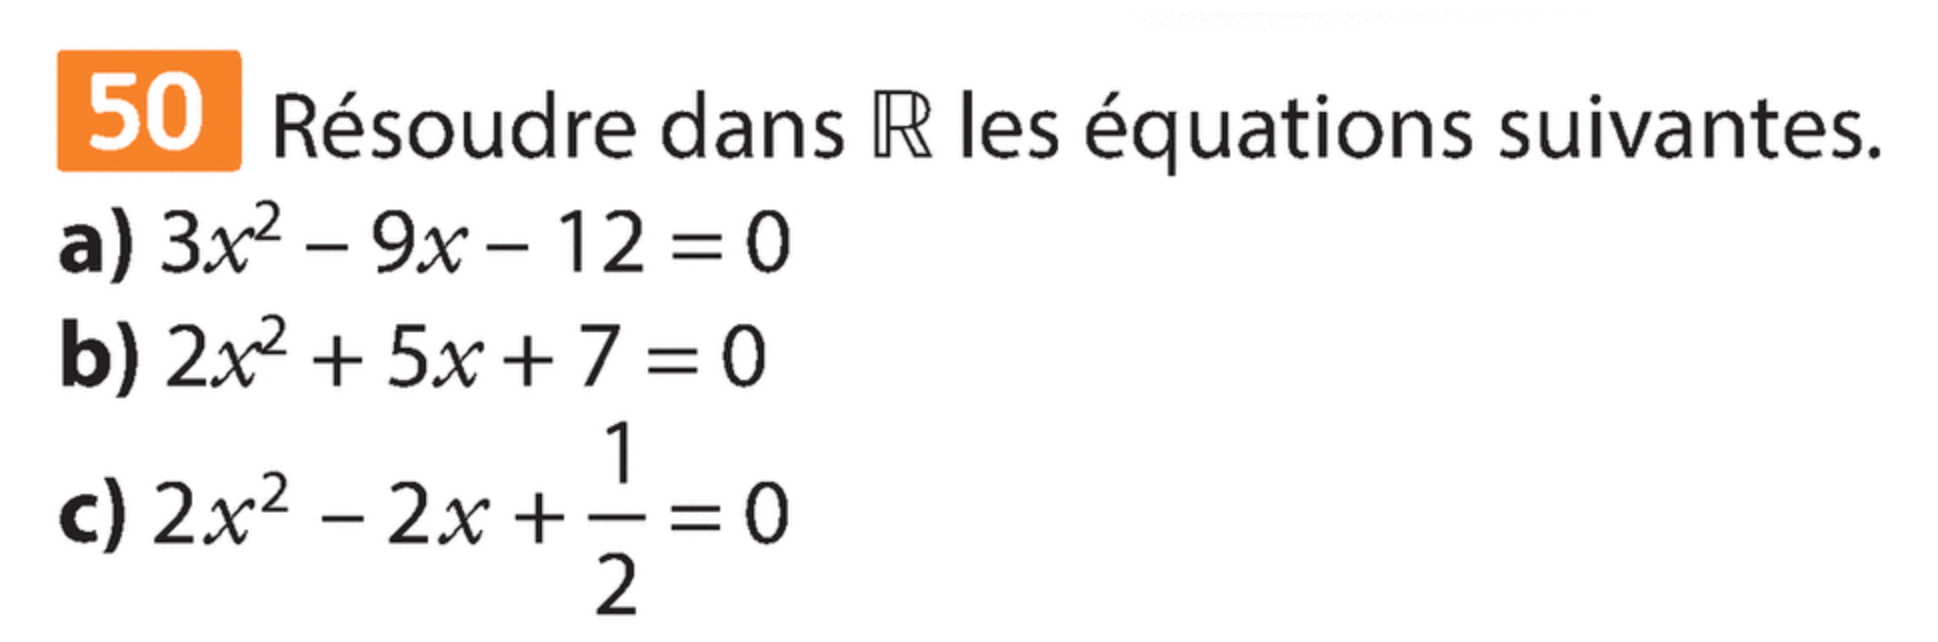
\includegraphics[scale=0.25]{01.DM01.Img03}

\vspace{-0.5cm}
\exercice{ - Nombre dérivé - ( 3 point )}

Soit $f$ la fonction définie sur $\mathbb{R}$ par $f: x \mapsto x^{2}+1$ et $h$ un nombre réel non nul.
\begin{enumMet}
    \item Exprimer en fonction de $h$ le taux de variation de $f$ entre 3 et $3+h$
    \item En déduire que la fonction est dérivable en 3 et déterminer $f^{\prime}(3)$.
    \item De la même manière, montrer que $f$ est dérivable en 2 et déterminer $f^{\prime}(-2)$.
\end{enumMet}
%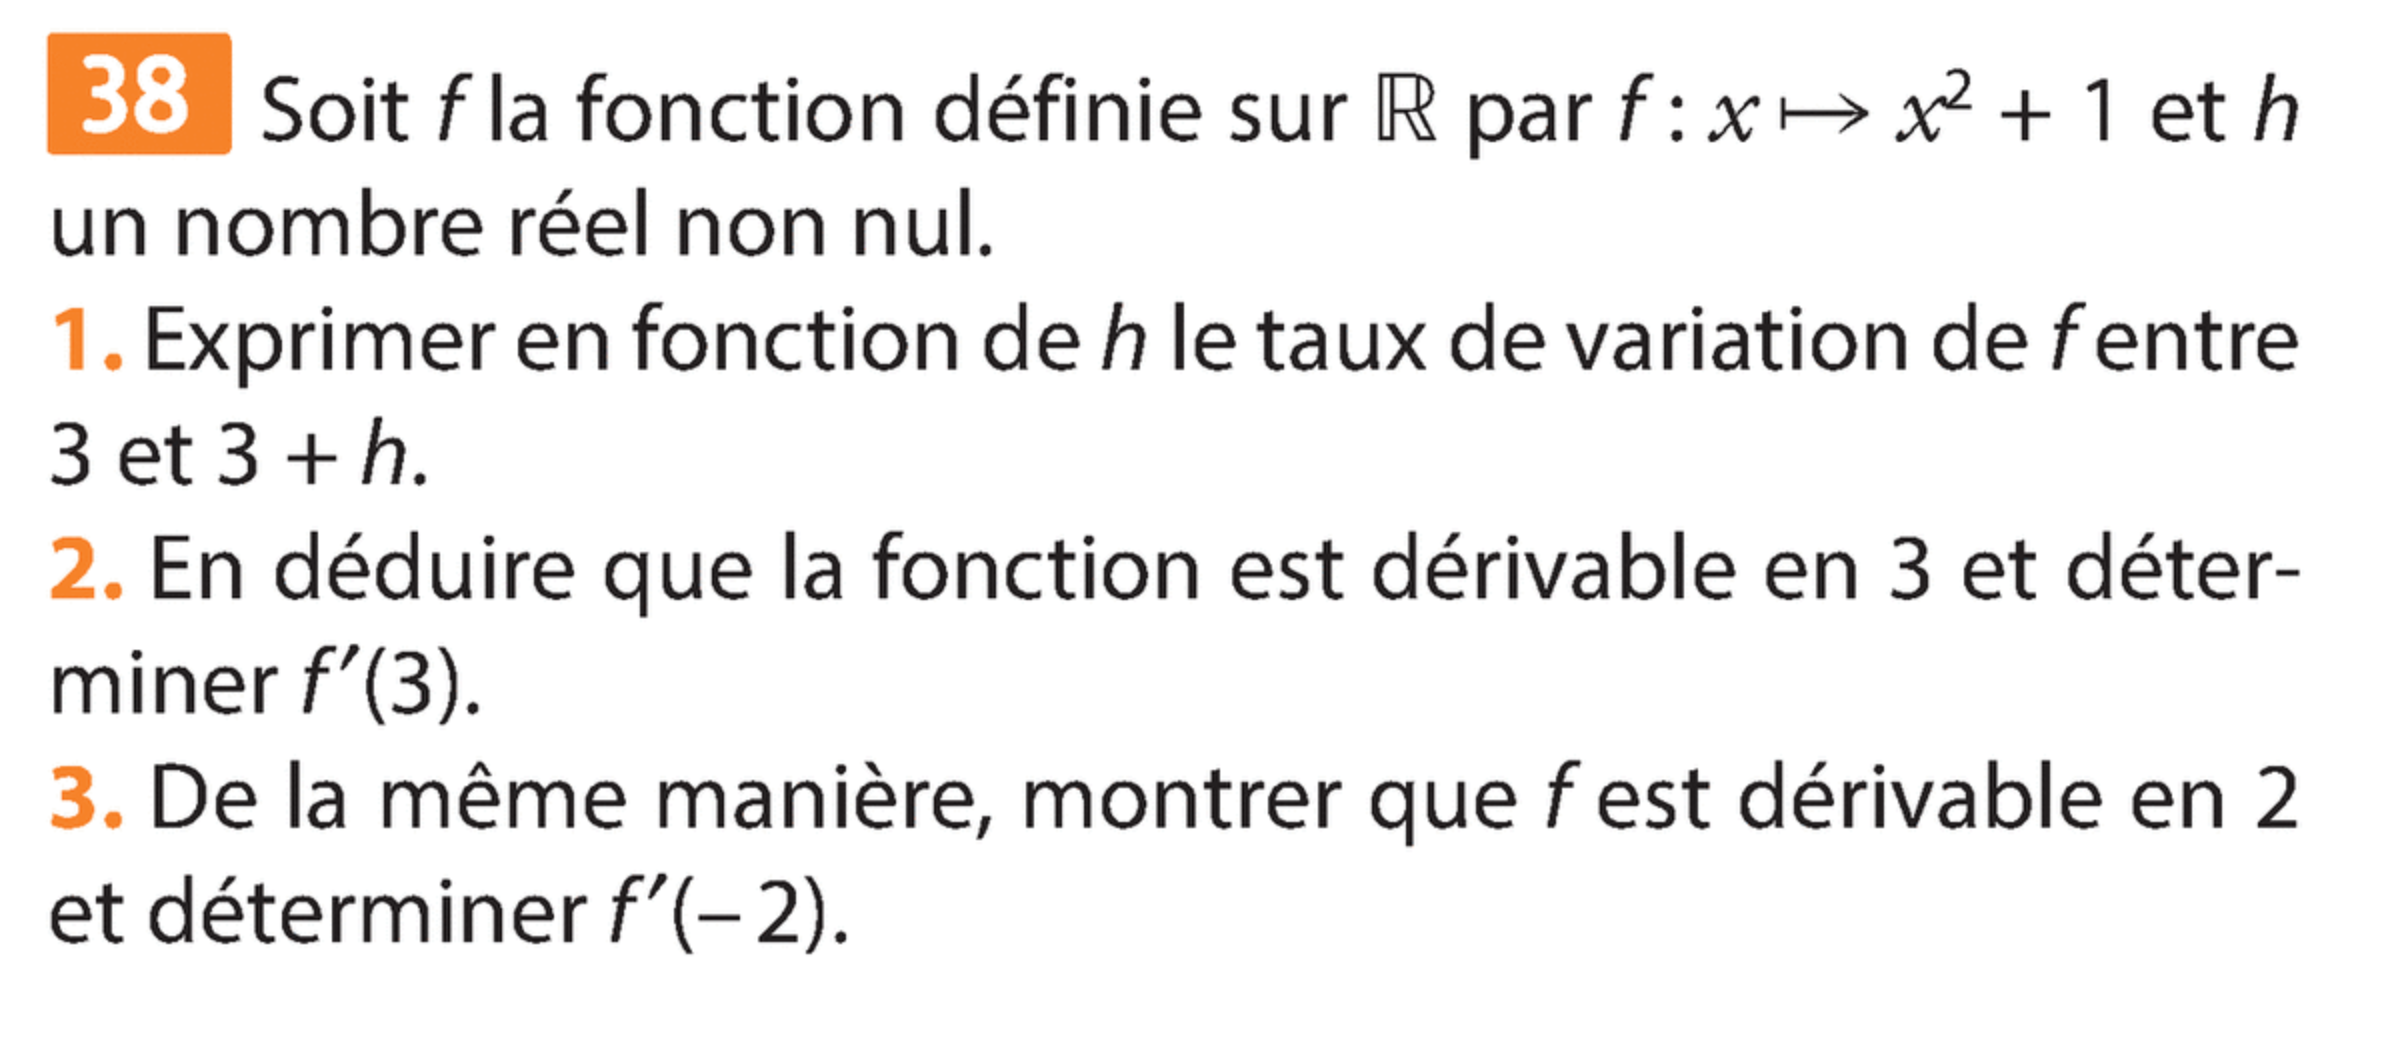
\includegraphics[scale=0.23]{01.DM01.Img04}


%\vspace{-0.6cm}
\exercice{ - tangentes et nombres dérivés - ( 6 point )}
\begin{multicols}{2}
Dans le repère orthonormé $(\mathrm{O} ; \vec{i}, \vec{j})$ ci-contre, la courbe rouge $\mathscr{C}_{f}$ représente une fonction $f$ définie et dérivable sur $\mathbb{R}$, les droites tracées en bleu représentent les tangentes à $\mathscr{C}_{f}$ respectivement au point $\mathrm{O}$, au point $\mathrm{B}$ d'abscisse 1 et au point $C$ d'abscisse 3
\begin{enumMet}
    \item Déterminer graphiquement $f^{\prime}(0), f^{\prime}(1)$ et $f^{\prime}(3)$
    \item Déterminer l'équation réduite de la tangente à $C_{f}$ au point $C$.
    \item La courbe $\mathscr{C}_{f}$ est la représentation graphique de la fonction $f: x \mapsto x^{3}-4 x^{2}+2 x$\\
    Retrouver par le calcul les résultats des questions 1) et 2)
\end{enumMet}

\columnbreak
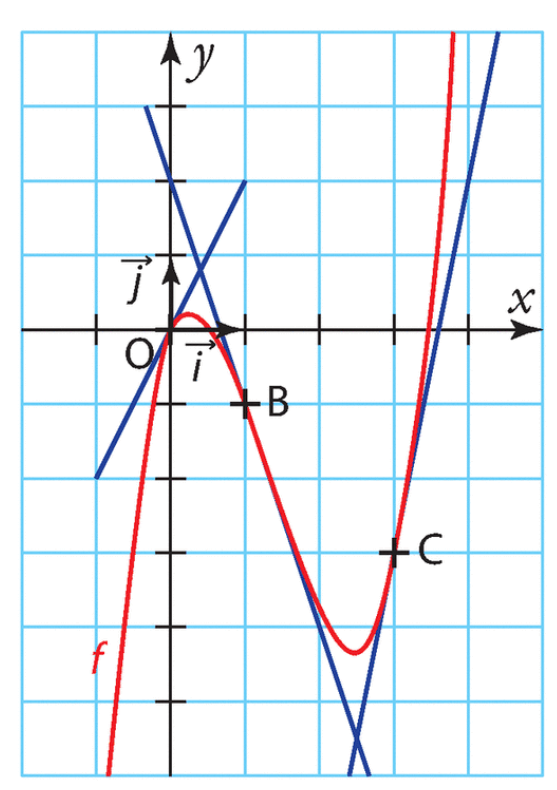
\includegraphics[scale=0.7]{01.DM01.Img07}
\end{multicols}



%\vspace{-0.3cm}
\exercice{ - droites perpendiculaires - ( 2 point )}
Soit les points $A(-5 ;-2), M(1 ;-3), T(-1 ; 2)$ et $H(0 ; 8)$.\\
Montrer que les droites (MA) et (TH) sont perpendiculaires.
%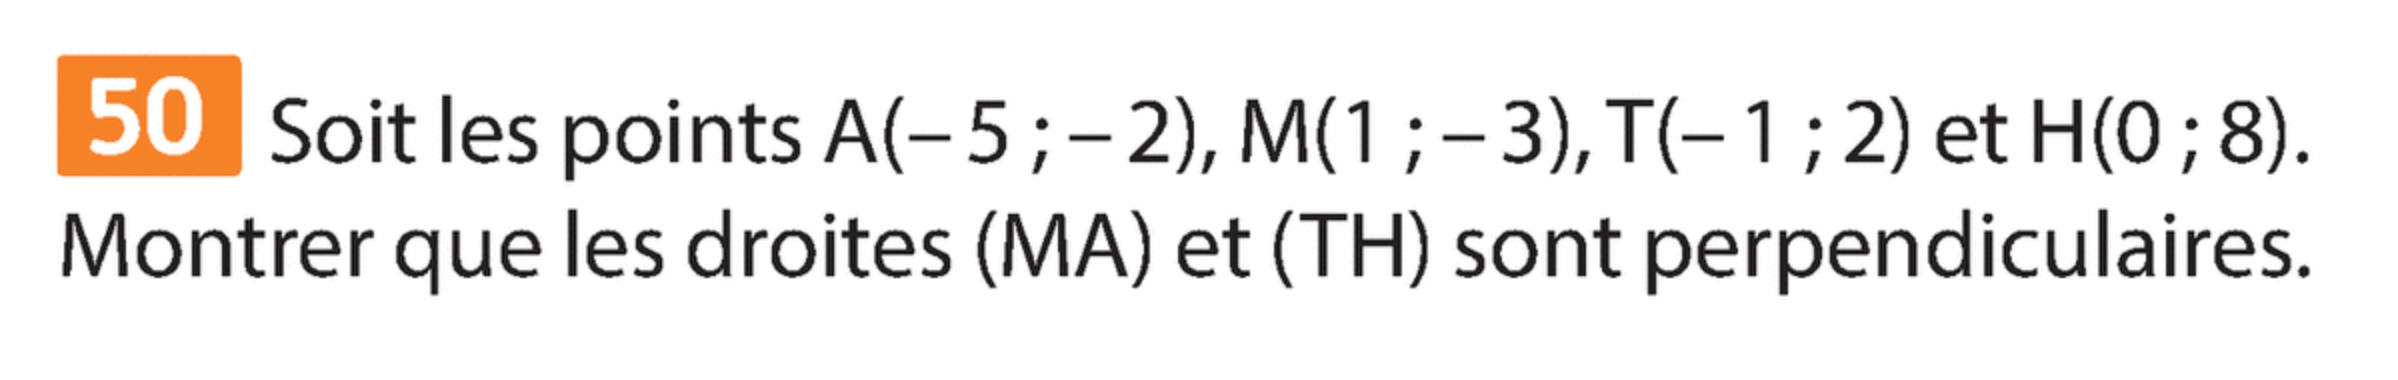
\includegraphics[scale=0.3]{01.DM01.Img11}

\newpage

%\vspace{-0.6cm}
\exercice{ - Fonction dérivée - ( 3 point )}

Déterminer pour chacune des fonctions suivantes sa fonction dérivée sur $\mathbb{R}$.
\begin{enumMet}
    \item $f(x)=\dfrac{3 x^{4}}{8}-\dfrac{5 x^{3}}{3}+2 x-\dfrac{11}{2}$
    \item $g(x)=\dfrac{x^{2}+x-1}{2x}$
    \item $h(x)=\dfrac{2}{x-3}$
\end{enumMet}
%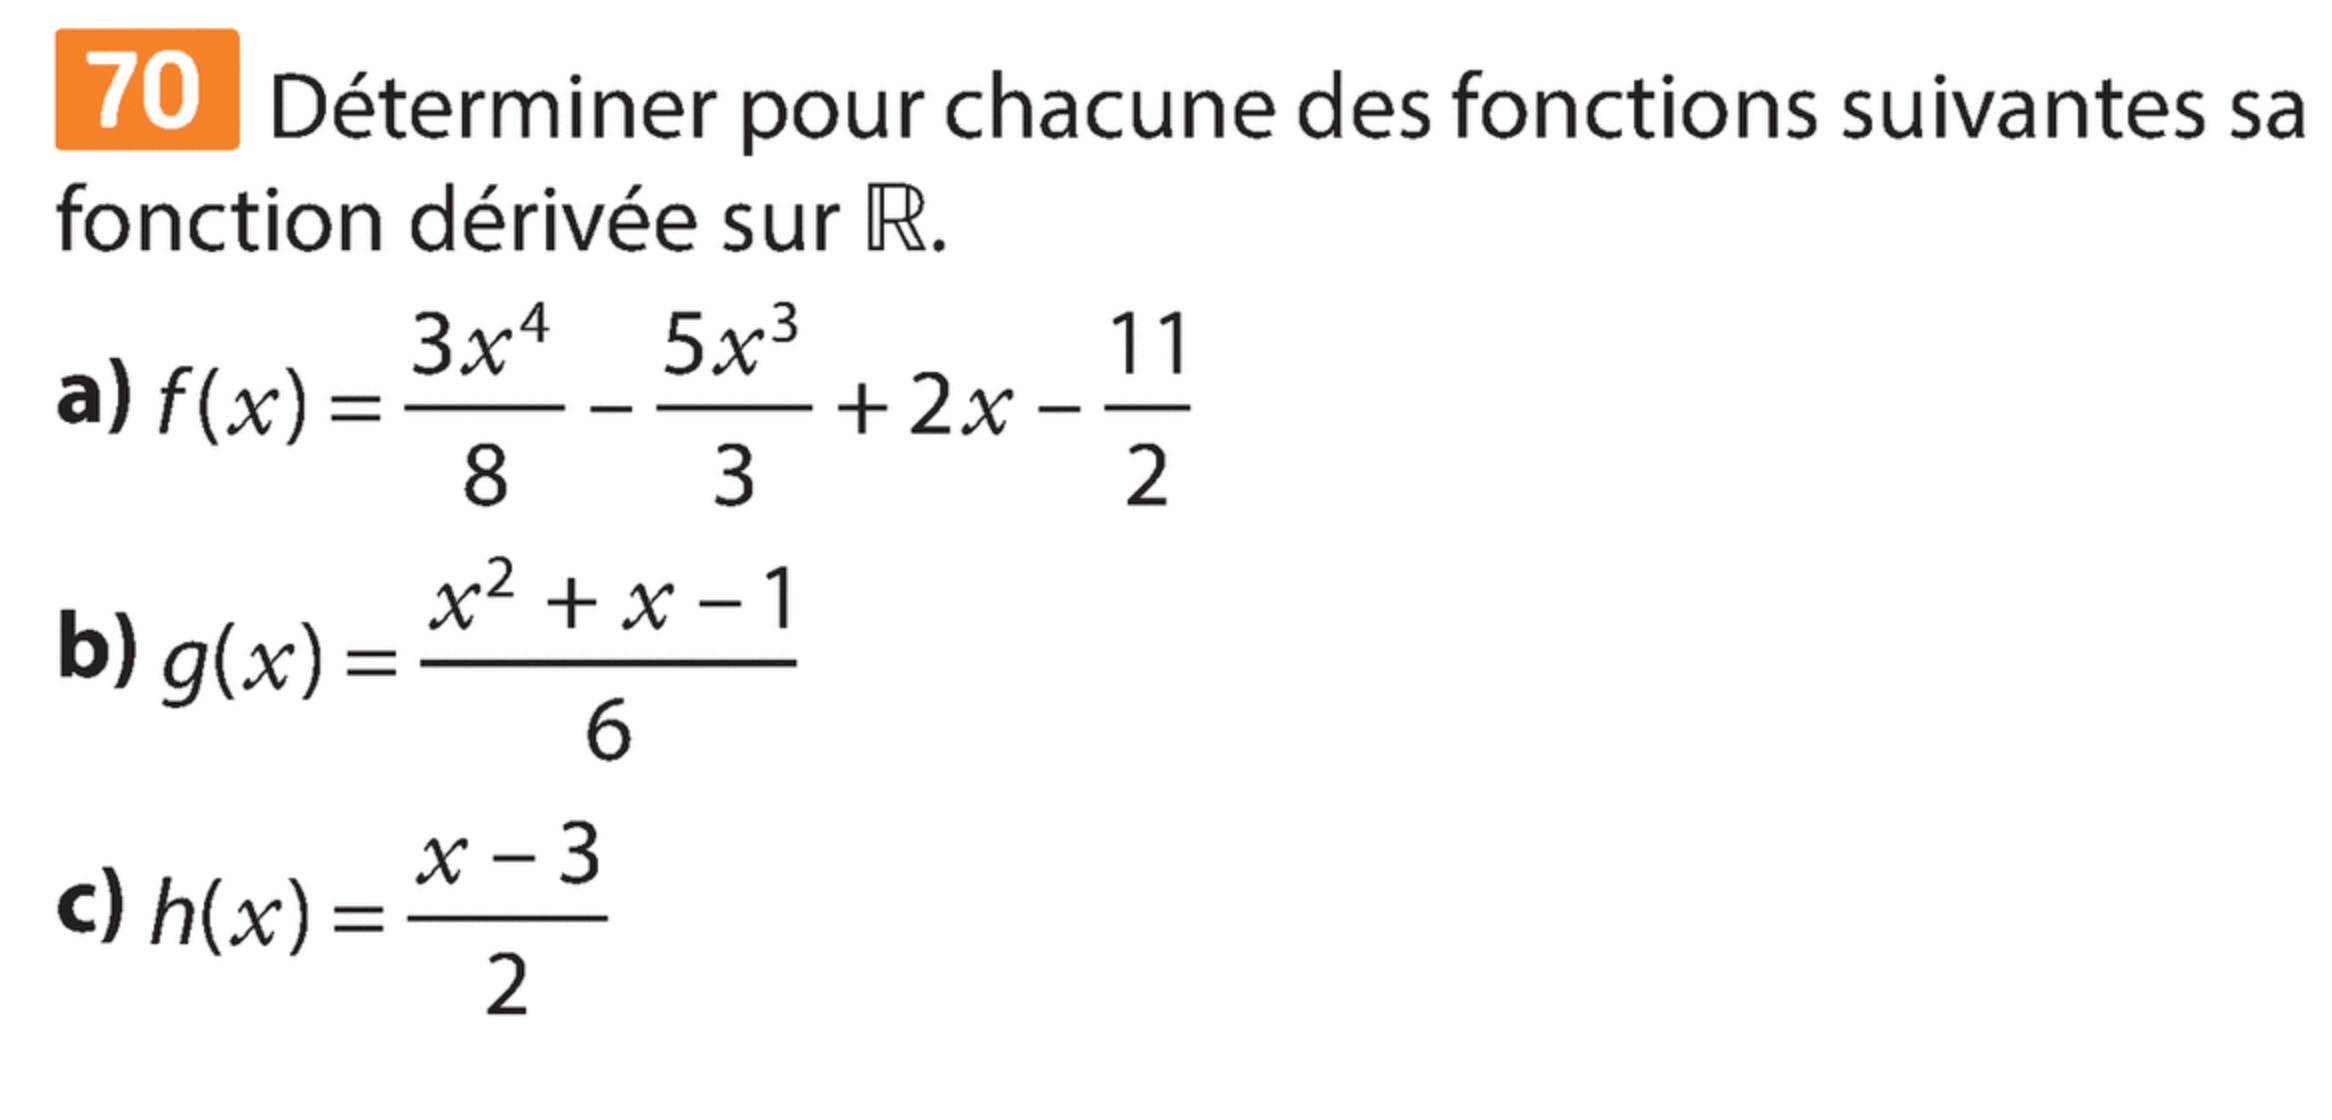
\includegraphics[scale=0.28]{01.DM01.Img06}

%\vspace{-0.6cm}
\exercice{ - projeté orthogonal - ( 6 point )}

ABCD est un carré de côté $8$, BEC est un triangle équilatéral extérieur au carré et I est le milieu du segment [BC].
\begin{enumMet}
    \item Calculer les produits scalaires suivants.
    \begin{multicols}{4}
        \begin{enumMet}
            \item $\overrightarrow{\mathrm{AC}} \cdot \overrightarrow{\mathrm{AB}}$
            \item $\overrightarrow{\mathrm{AB}} \cdot \overrightarrow{\mathrm{DC}}$
            \item $\overrightarrow{\mathrm{AB}} \cdot \overrightarrow{\mathrm{DB}}$
            \item $\overrightarrow{\mathrm{AC}} \cdot \overrightarrow{\mathrm{BD}}$
        \end{enumMet}
    \end{multicols}
    \item Calculer également $\overrightarrow{\mathrm{BC}} \cdot \overrightarrow{\mathrm{BE}}$ et $\overrightarrow{\mathrm{CE}} \cdot \overrightarrow{\mathrm{BC}}$.
    \item On rappelle que la hauteur du triangle équilatéral vaut $4 \sqrt{3}$\\
    Calculer alors les produits scalaires suivants.
    \begin{multicols}{3}
        \begin{enumMet}
            \item $\overrightarrow{\mathrm{AB}} \cdot \overrightarrow{\mathrm{BE}}$
            \item $\overrightarrow{\mathrm{CE}} \cdot \overrightarrow{\mathrm{CD}}$
            \item $\overrightarrow{\mathrm{BA}} \cdot \overrightarrow{\mathrm{E}}$
        \end{enumMet}
    \end{multicols}
\end{enumMet}

%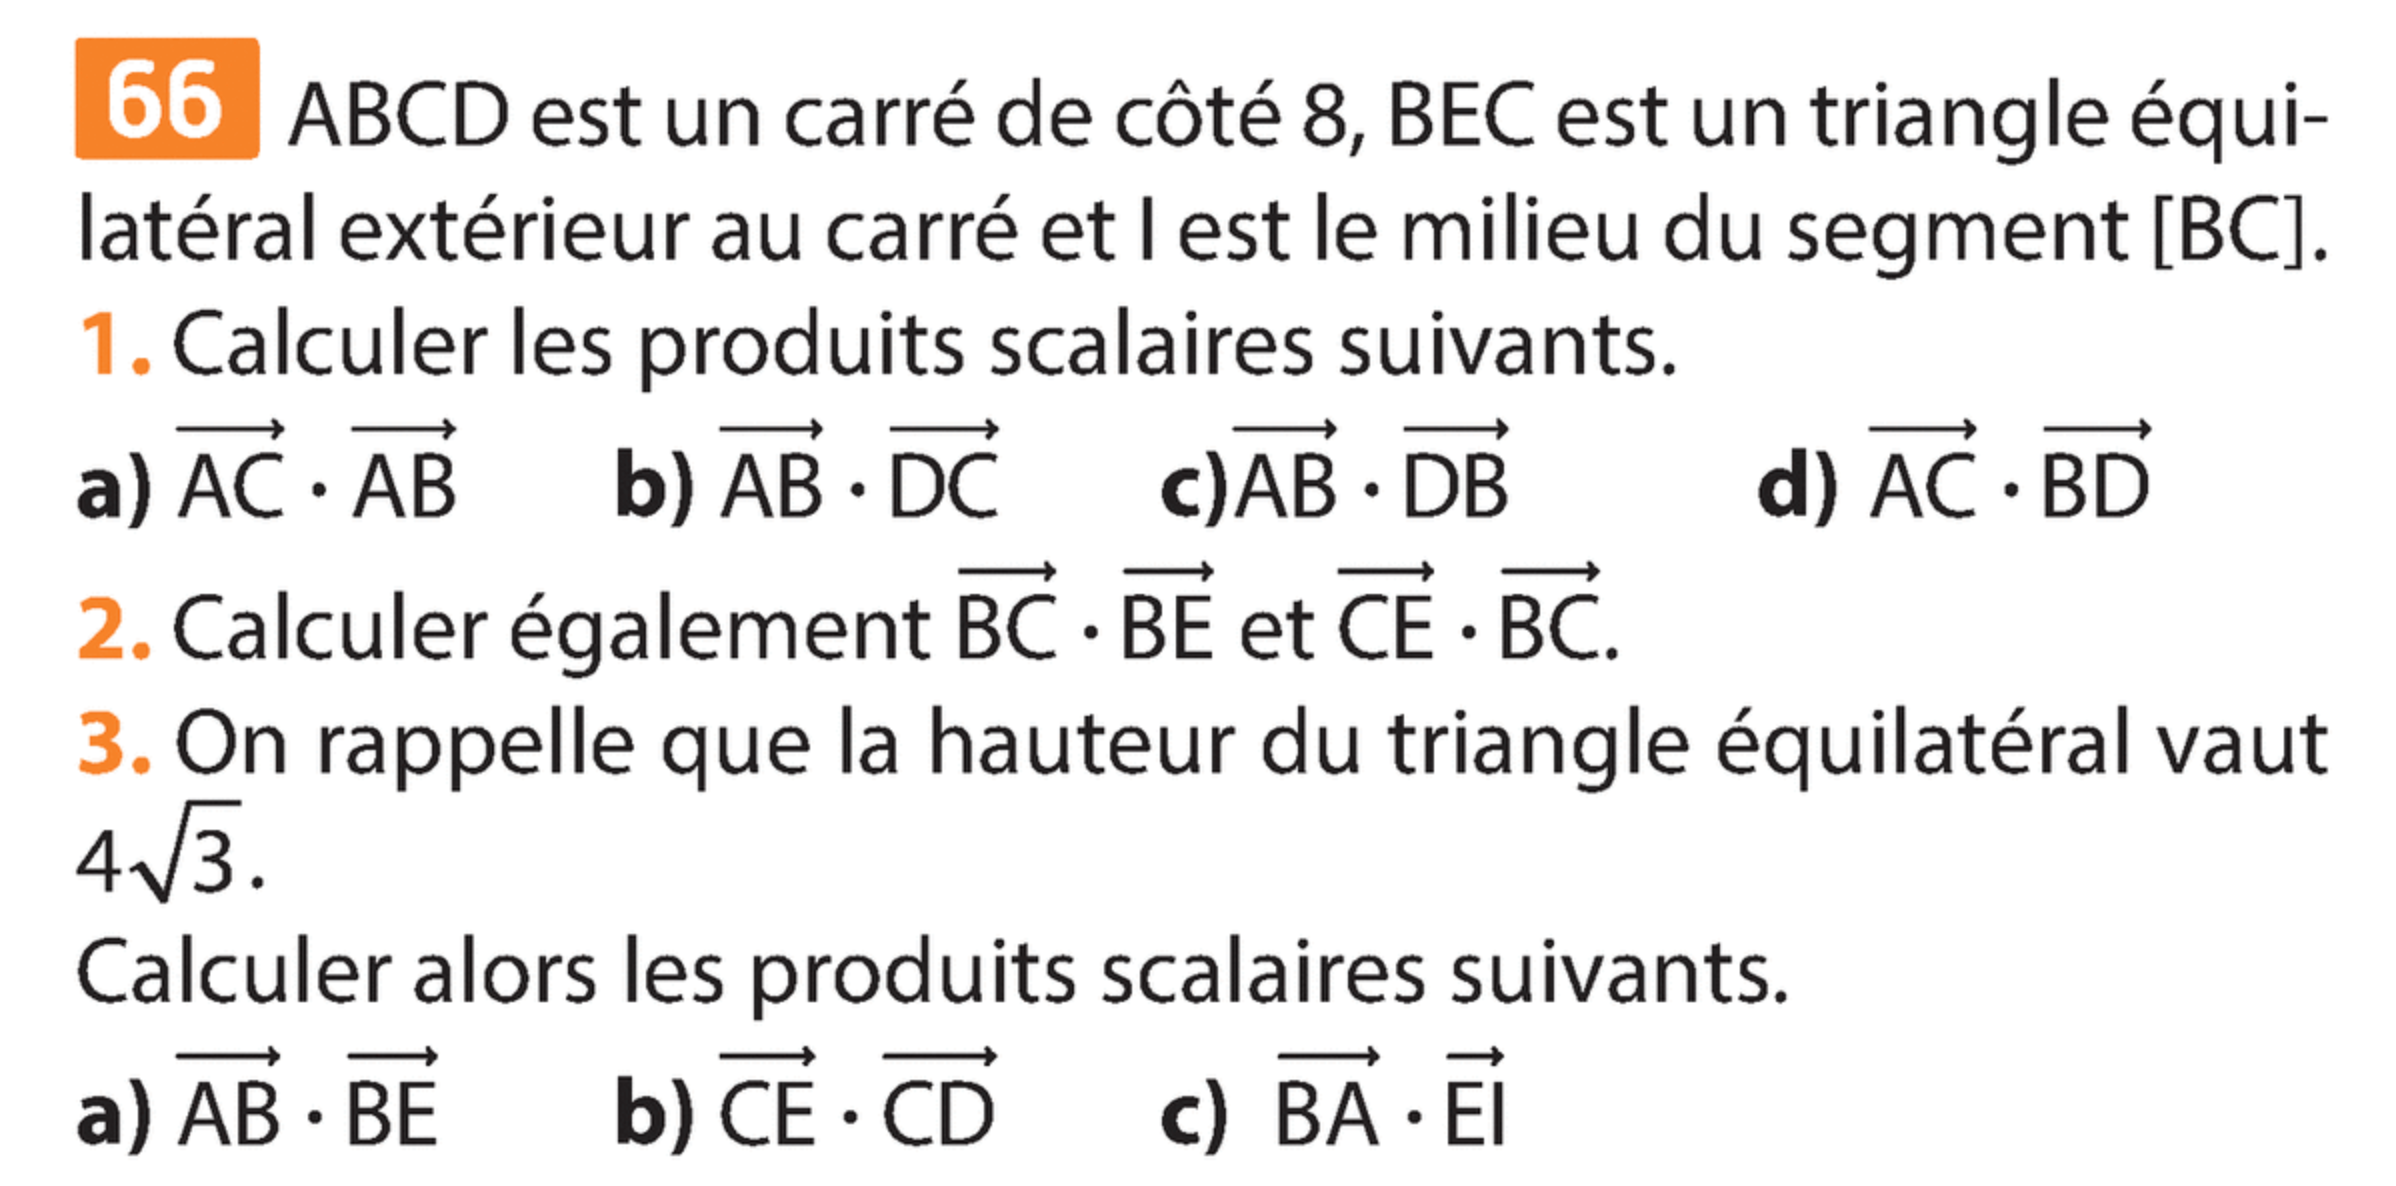
\includegraphics[scale=0.28]{01.DM01.Img10}

%\vspace{-0.6cm}
\exercice{ - Produit scalaire et repère - ( 6 point )}
Soit les vecteurs $\vec{u}\left(\begin{array}{l}2 \\ 1\end{array}\right), \vec{v}\left(\begin{array}{c}-3 \\ -1\end{array}\right)$ et $\vec{w}\left(\begin{array}{l}1 \\ 4\end{array}\right)$\\
Calculer les produits scalaires suivants.
\begin{multicols}{2}
\begin{enumMet}
    \item $\vec{u} \cdot \vec{v}$
    \item $\vec{w} \cdot \vec{v}$
    \item $\vec{u} \cdot(\vec{v}+\vec{w})$
    \item $(-2 \vec{u}) \cdot \vec{v}+3(\vec{v} \cdot \vec{w})$
\end{enumMet}
\end{multicols}
%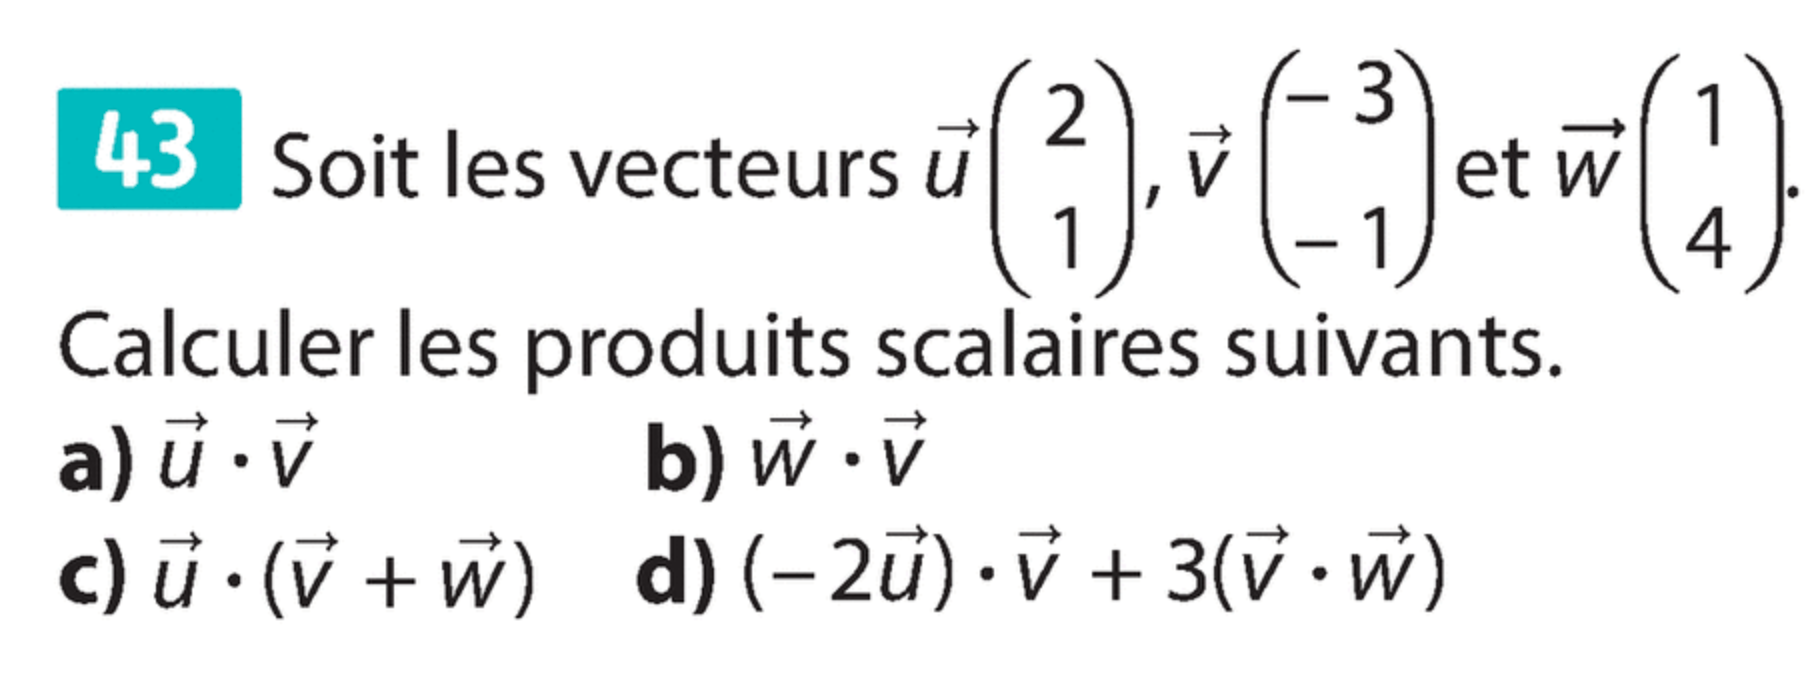
\includegraphics[scale=0.3]{01.DM01.Img12}

%\vspace{-0.6cm}
\exercice{ - équation cartésienne - ( 4 point )}
On considère la droite $d$ d'équation cartésienne $-5 x+3 y-1=0$
\begin{enumMet}
    \item Donner un vecteur directeur de $d$.
    \item En déduire un vecteur normal de $d$.
    \item Donner une équation cartésienne de la droite $d^{\prime}$ perpendiculaire à $d$ passant par le point $F(2 ;-2)$.
    \item Donner une équation réduite de la droite $d^{\prime}$.
\end{enumMet}
%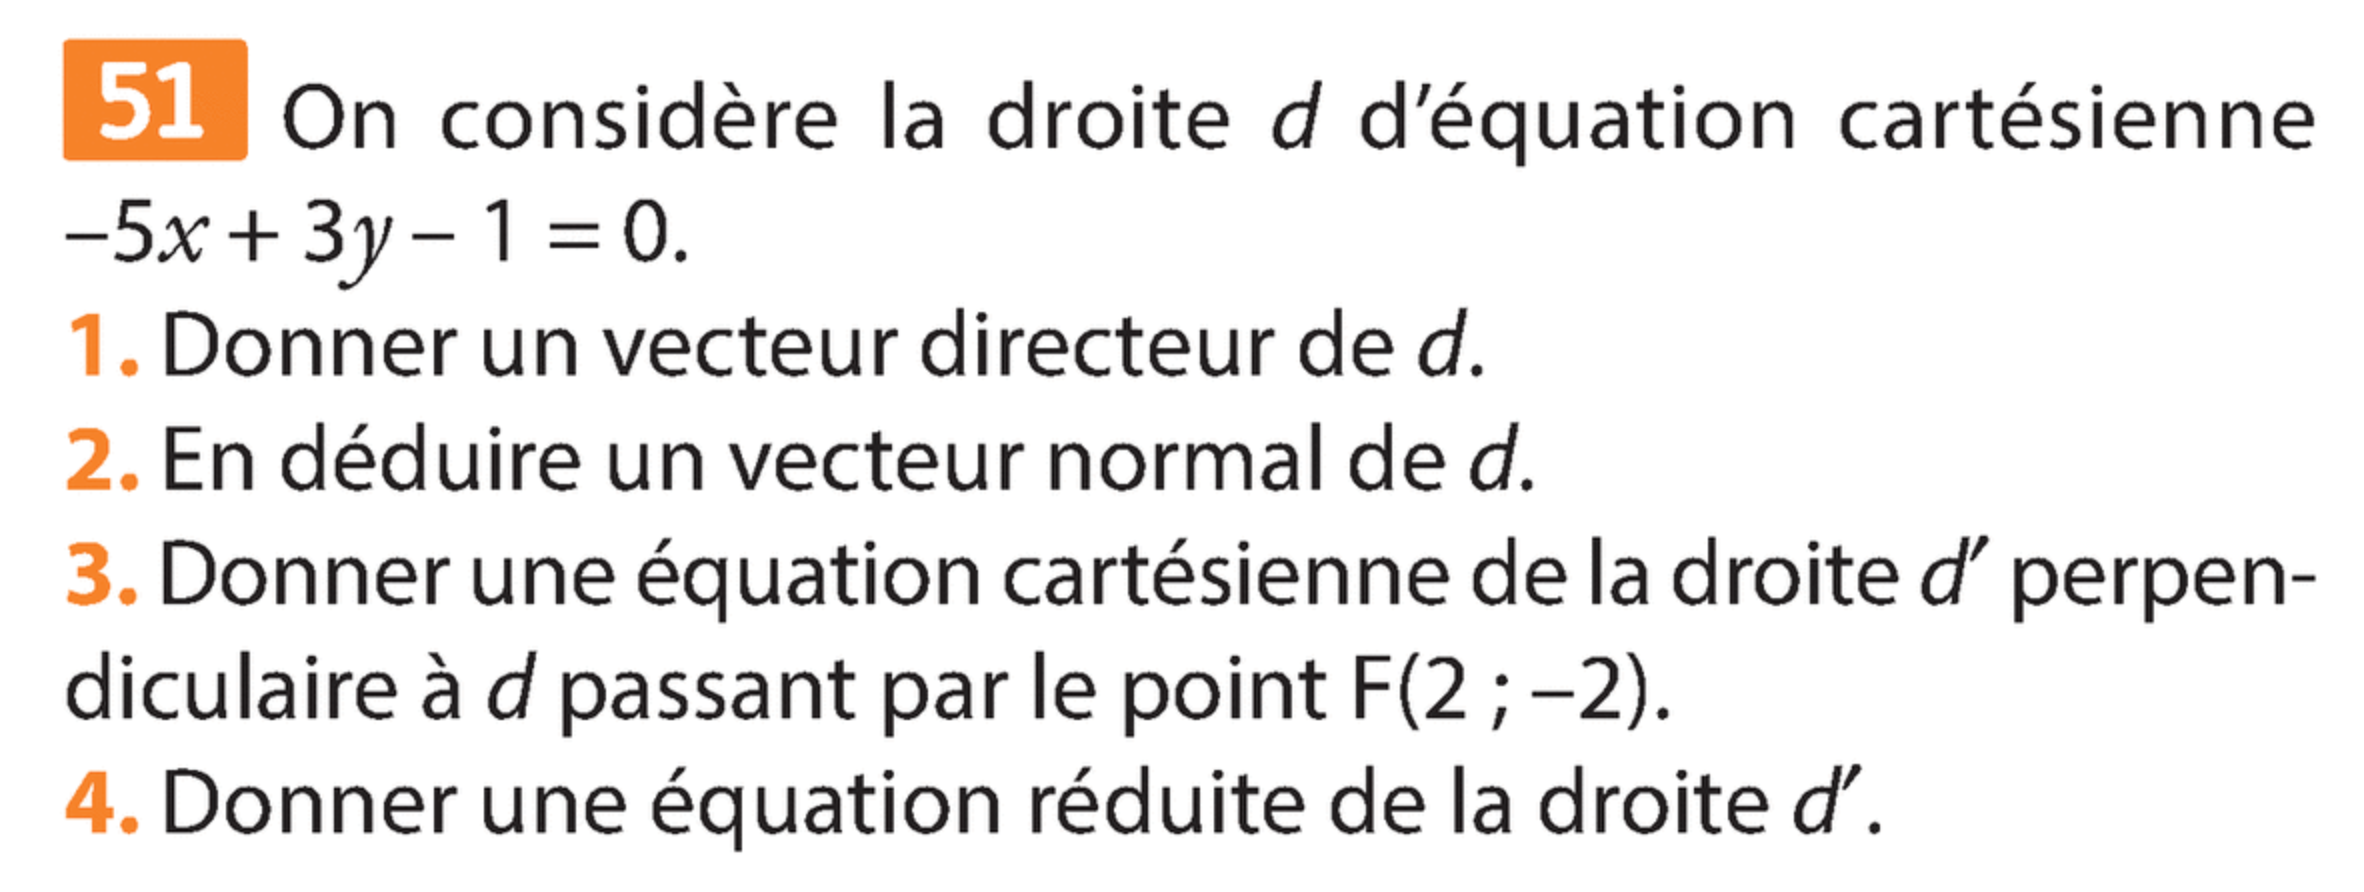
\includegraphics[scale=0.28]{01.DM01.Img14}

%\vspace{-0.6cm}
\exercice{ - Théorème d'Al Kashi - ( 2 point )}

On considère les points $M, N$ et $P$ tels que $M N=5,$ $\mathrm{NP}=7$ et $\widehat{\mathrm{MNP}}=61^{\circ}$.\\
Déterminer la longueur MP.
%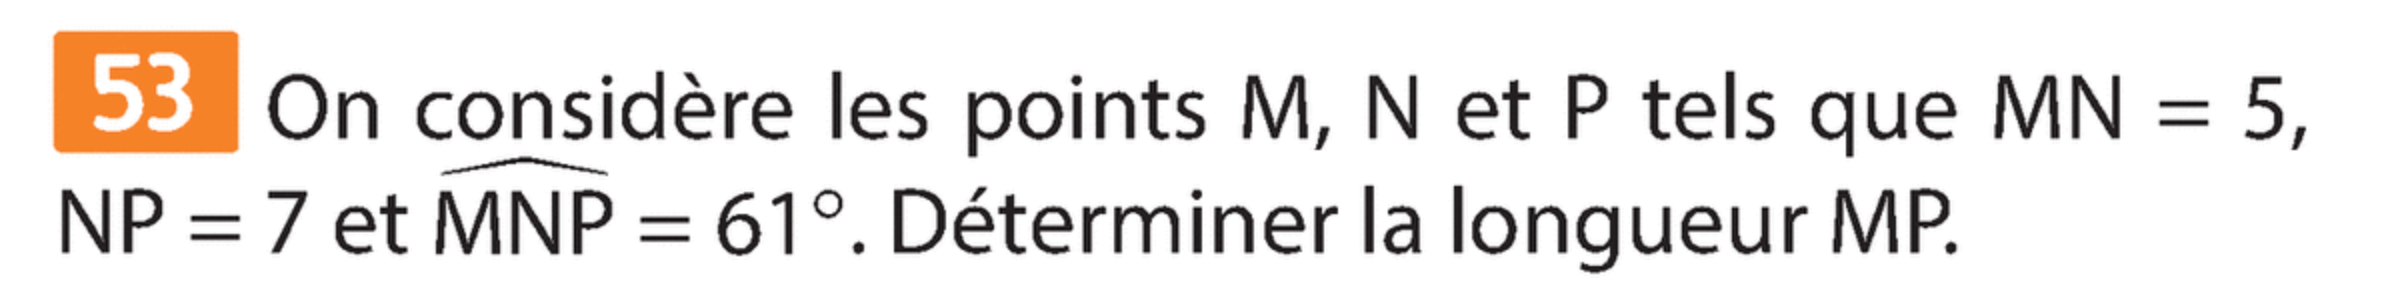
\includegraphics[scale=0.28]{01.DM01.Img15}

\end{document}

